\section{仿真实验与结果}\label{sec:new-experiments}
\subsection{固定协议、独立调参与计时口径}
新增实验在共享 Linux 服务器执行：主机为双路 Intel Xeon 6759P-C，共 240 个逻辑核；图像训练只使用一张 NVIDIA H20-3e（143,771 MiB 显存）与 4 个绑定的 CPU 线程，矩阵分解采用 CPU float64。图像训练采用 float32、channels-last，关闭 TF32，PyTorch 为服务器已有的 2.8.0a0 版本，CUDA 为 12.9。原有精确二次问题、随机梯度与微型语言模型记录保留在附录，仍可追溯到不可变的 \texttt{v1.0} 版本。迁移前的未完成 CPU 图像记录不纳入本节统计。新增实验的随机种子为 $0,1,2$，报告均值与样本标准差；试跑种子 42 与正式种子分开。

为控制共享机器负载，所有图像运行串行执行，PyTorch 显存分配器上限设为设备显存的 4\%，每步及每个评价批次后主动等待，使计算占空目标为 35\%。该等待策略不是硬件算力配额；共享任务仍会影响实际耗时。若设备全局剩余显存低于 12 GiB，程序在检查点退出自身任务。进程使用较低 CPU 与 I/O 优先级，不改变设备的全局设置。计时区分同步后的单步活跃时间与包含主动等待的训练墙钟，不能把后者解释成独占 H20 的吞吐量。

三个优化器各有三个学习率候选，按相同短程预算独立选择。因子分解按试跑末点目标值选取，图像分类按试跑末点验证交叉熵选取。这里的“选定”只表示所列离散候选中的最佳值，不声称得到全局最优超参数。数据、模型初始化、批次顺序、增强随机序列和调度器在同一种子下保持一致；正式协议在读取正式测试结果之前冻结。

\subsection{\texorpdfstring{条件数 $10^4$}{条件数 10000} 的非凸矩阵分解}
构造满秩目标 $A=P\operatorname{diag}(s_i)R^\top\in\mathbb R^{32\times32}$，其中 $P,R$ 为正交矩阵，$s_i$ 从 1 到 $10^{-4}$ 按几何间隔排列，故 $\kappa_2(A)=10^4$。实际优化两个矩阵因子：
\begin{equation}\label{eq:factorization}
 \min_{U,V\in\mathbb R^{32\times32}}
 F(U,V)=\frac12\|UV^\top-A\|_F^2.
\end{equation}
其梯度分别为 $(UV^\top-A)V$ 与 $(UV^\top-A)^\top U$。相对重构误差定义为 $\|UV^\top-A\|_F/\|A\|_F$，图中梯度核范数为两个参数块核范数之和。双因子乘积使目标成为四次非凸函数；目标奇异值条件数不等于 Hessian 条件数。

三个方法各有三个学习率候选：SGD+M 为 $\{0.03,0.1,0.3\}$，AdamW 为 $\{0.001,0.01,0.05\}$，Muon 为 $\{0.005,0.02,0.05\}$。试跑 300 步，正式运行 3000 步。所有方法关闭权重衰减；SGD 动量为 0.9，AdamW 的矩参数为 $(0.9,0.95)$，Muon 使用 0.95 的普通 EMA 与五步 NS。因子初值为同种子的零均值高斯矩阵，元素标准差 0.03。

\begin{figure}[htbp]\centering
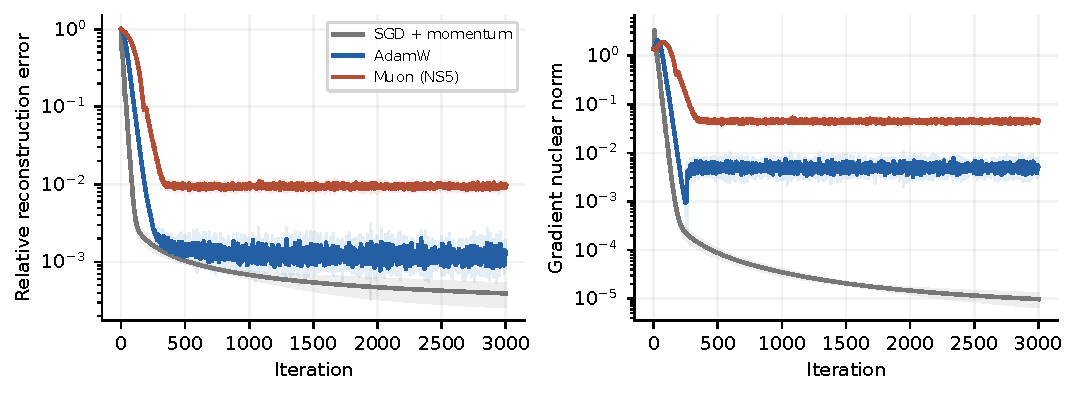
\includegraphics[width=\linewidth]{fig1.pdf}
\caption{非凸病态矩阵分解：相对重构误差与真实梯度核范数。曲线为三个种子的均值，阴影为样本标准差；两图均用对数纵轴。}\label{fig:factorization-new}
\end{figure}

本次矩阵分解中，普通动量 SGD 获得更低的末点重构误差；Muon 的归一化常步长在末段留下残差。因此，病态目标本身并不构成“Muon 必然加速”的证据。该四次因子目标只有局部光滑性，且存在因子缩放不唯一性，不能不加条件地代入全局光滑定理。附录中的固定二次问题才是与原始理论假设直接对应的受控数值检查。

\subsection{CIFAR-10 与完整 ResNet-18}
CIFAR-10 的官方数据包含 50,000 张训练图和 10,000 张测试图\citep{cifar2009}。从官方训练部分按类别分层保留 5,000 张作验证，其余 45,000 张用于训练。划分种子、图像数和索引摘要记录在数据清单中；下载的官方二进制压缩包先核对发布页的 MD5，再解析像素，不反序列化 pickle。

模型严格采用 ResNet-18 的 $[2,2,2,2]$ 基本块结构与 $[64,128,256,512]$ 通道宽度\citep{resnet2016}，保留原始 $7\times7$、步长 2 的输入卷积及 max-pool，只把分类层改为 10 类，共 11,181,642 个参数。输入使用原始 $32\times32$ 图像；这与常见的 $3\times3$ stem CIFAR 变体不同，空间分辨率下降更早。所有方法使用相同结构，不与采用另一种 stem 的公开准确率作直接比较。

训练增强为四像素补零、随机裁剪与水平翻转，再按固定通道均值和标准差归一化。批量 128，正式训练 3 个 epoch，共 1056 次更新，前 50 步预热，之后余弦下降到初始学习率的 0.1 倍。本实验是完整数据上的短程 GPU 比较，不能据此推断充分训练后的最终准确率。

\begin{table}[htbp]\centering\footnotesize
\caption{固定超参数与硬件设置。偏置和归一化参数均不衰减；SGD 使用耦合 L2，两个自适应配置使用解耦衰减。}\label{tab:cifar-config}
\resizebox{\linewidth}{!}{\begin{tabular}{lccc}\toprule
配置项 & SGD+M & AdamW & Muon 混合 \\ \midrule
模型 / 参数量 & \multicolumn{3}{c}{完整 ResNet-18 / 11,181,642} \\
输入 / stem & \multicolumn{3}{c}{$32\times32$ / 原始 $7\times7$、步长 2，保留 max-pool} \\
训练 / 验证 / 测试 & \multicolumn{3}{c}{45,000 / 5,000 / 10,000} \\
批量 / epoch / 种子 & \multicolumn{3}{c}{128 / 3 / 0、1、2} \\
硬件 / 精度 & \multicolumn{3}{c}{单张 H20-3e，Xeon 6759P-C；float32、4 个 CPU 线程} \\
共享资源限制 & \multicolumn{3}{c}{GPU 分配器上限 4\%，协作占空目标 35\%，TF32 关闭} \\
选定学习率 & 0.03 & 0.003 & 0.05 \\
动量 / 矩参数 & $0.9$ & $(0.9,0.95)$ & $0.95$；辅助 AdamW $(0.9,0.95)$ \\
矩阵权重衰减 & $5\times10^{-4}$ & $5\times10^{-4}$ & $5\times10^{-4}$ \\
调度 / 调参预算 & \multicolumn{3}{c}{50 步预热、余弦衰减；各 3 个 LR、种子 42、96 步} \\
\bottomrule\end{tabular}
}
\end{table}

图像分类的 SGD、AdamW 与 Muon 学习率候选分别为 $\{0.03,0.1,0.3\}$、$\{0.0003,0.001,0.003\}$、$\{0.005,0.02,0.05\}$。各候选以种子 42 运行 96 步，使用完整验证集的交叉熵选择；辅助 AdamW 固定采用已选定的 AdamW 学习率。有限的短程候选搜索可能偏好早期表现较好的设置，这是协议的限制，不能将其描述为充分调参后的优化器排名。

每个 epoch 在验证集评价并保存检查点。全部训练结束后，才离线计算各 epoch 的测试指标以绘制曲线；检查点选择只使用验证交叉熵。三种主配置共 9 次正式训练，同一模型中其他训练规则不变。ReLU、BatchNorm 及按 epoch 无放回打乱的数据顺序均未被证明满足前述理论的全部条件；该实验报告实际应用结果，不充当定理假设的验证。

\begin{figure}[htbp]\centering
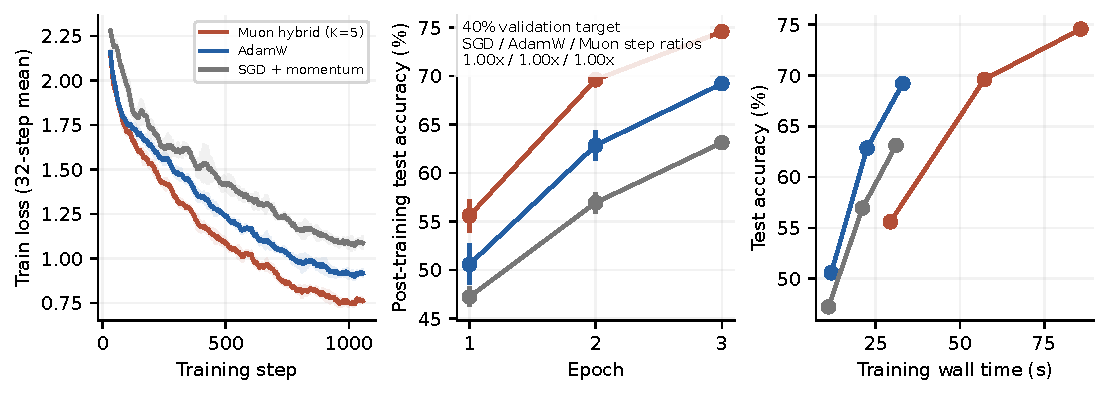
\includegraphics[width=\linewidth]{fig2.pdf}
\caption{CIFAR-10 短程训练。左图训练损失采用 32 步滑动平均；中图为训练后离线测试准确率，误差棒为三个种子的样本标准差；右图横轴包含实际训练、验证、谱诊断及主动等待，不包含后验测试与进程启动。图中步数比使用验证集 40\% 阈值，不能由测试曲线反向选阈值。}\label{fig:cifar-dynamics}
\end{figure}

达标阈值预先固定为验证准确率 40\%，只在 epoch 末检查。达标步数因此具有 352 步的分辨率；没有达到阈值时记为未达标，不用总预算代替首次达标步数。“步数比”定义为同种子 SGD 达标步数除以该方法达标步数；仅在两者均达标时计算，三对结果不全可用时不报告一个掩盖失败样本的平均加速比。

\begin{table}[htbp]\centering\footnotesize
\caption{CIFAR-10 三种子结果。准确率来自验证损失选定的检查点；步数比只衡量样本效率。单步耗时为 CUDA 同步后的活跃时间中位数，不含主动等待。RSS 为独立进程峰值，显存为 PyTorch 峰值已分配量，不含 CUDA 上下文；缓存保留量另存原始日志。}\label{tab:cifar-performance}
\setlength{\tabcolsep}{3pt}
\resizebox{\linewidth}{!}{\begin{tabular}{lccccccc}\toprule
方法 & 末轮 Loss & Acc / \% & 达标步数 & 步数比 & ms/step & RSS / MiB & 显存 / MiB \\ \midrule
SGD+M & $1.136\pm0.010$ & $63.12\pm0.39$ & $352\pm0$ & $1.0\pm0.0$ & $9.3\pm0.0$ & $1523\pm0$ & $254\pm0$ \\
AdamW & $0.957\pm0.012$ & $69.21\pm0.11$ & $352\pm0$ & $1.0\pm0.0$ & $9.9\pm0.0$ & $1594\pm0$ & $295\pm0$ \\
Muon 混合 & $0.798\pm0.008$ & $74.57\pm0.27$ & $352\pm0$ & $1.0\pm0.0$ & $26.8\pm0.2$ & $1618\pm0$ & $255\pm0$ \\
\bottomrule\end{tabular}
}
\end{table}

本次 SGD+M、AdamW 与 Muon 混合配置的选定测试准确率均值分别为 \CifarSGDAcc\%、\CifarAdamAcc\% 与 \CifarMuonAcc\%；对应单步耗时中位数的种子均值为 \CifarSGDStep、\CifarAdamStep\ 和 \CifarMuonStep\ 毫秒。图\ref{fig:cifar-dynamics}与表\ref{tab:cifar-performance}分别呈现按步数和实际时间评价的结果；二者不必给出相同排序。

本次 Muon 的准确率更高，单步活跃时间也更长。三种方法的三个种子均在首次 epoch 检查时达到 40\% 验证阈值，配对步数比均为 1，因此该阈值没有检测到步数优势。这也说明较低阈值与较粗的检查间隔会限制加速指标的区分能力。

\subsection{更新矩阵奇异值谱与机理边界}
选择固定的隐藏卷积参数 \texttt{layer1.0.conv2.weight}，展平为 $64\times576$ 矩阵，记录第 1 步与每个 epoch 末的真实权重差 $\Delta W_t=W_t-W_{t+1}$。该量包含实际优化器方向及权重衰减。各方法使用同一参数层和检查时刻，不挑选谱图更好看的层。归一化谱为 $s_i/s_1$；有效条件数只使用超过 $\max(10^{-6}s_1,10^{-12})$ 的奇异值，并同时保存数值秩。

\begin{figure}[htbp]\centering
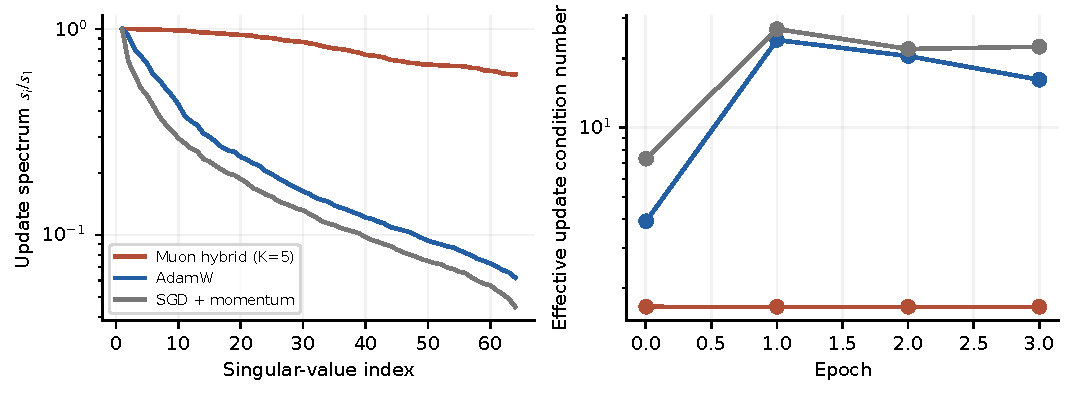
\includegraphics[width=\linewidth]{fig3.pdf}
\caption{代表层实际更新的谱。左图使用末次更新的归一化奇异值，再跨种子平均；右图为预先规定容差下的有效条件数。观察对象是权重更新，不能由此证明激活特征坍缩被消除。}\label{fig:update-spectrum}
\end{figure}

对精确极因子，非零支撑上的奇异值均为 1，这个代数事实解释了谱均衡机制。实际五步多项式、动量、衰减和浮点差分共同影响记录到的更新谱。条件数变小只能说明该更新的谱更均衡；表示层特征是否退化还需要激活协方差、表示秩等额外测量，不能用一幅更新谱图代替。

\subsection{\texorpdfstring{$K=0,1,3,5,7$}{K=0,1,3,5,7} 的训练消融}
对五个 $K$ 值各运行三个种子，共 15 次 Muon 训练，其中 $K=5$ 与主比较共享记录，因此图像分类正式训练总数为 21 次。消融固定 $K=5$ 试跑所选的学习率、辅助 AdamW、初始化、数据增强和训练预算，仅改变多项式次数。$K=0$ 表示仅做 Frobenius 归一化，仍有动量和非零更新。

\begin{figure}[htbp]\centering
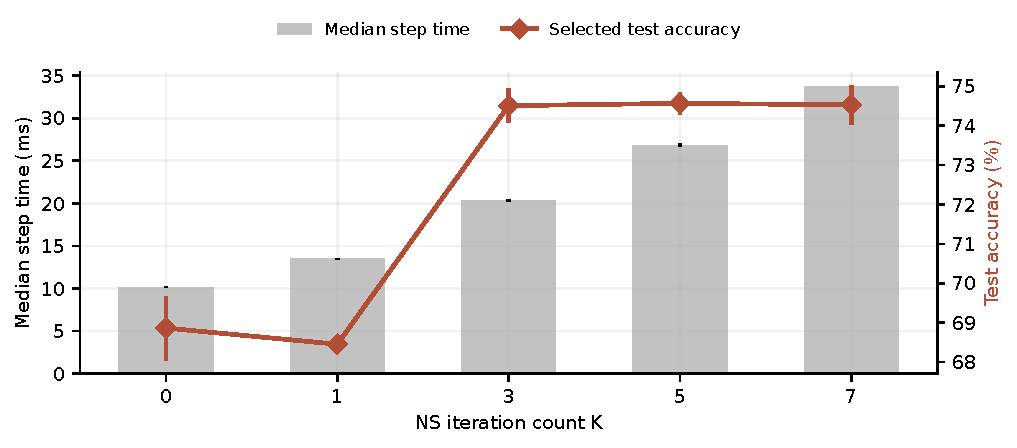
\includegraphics[width=.95\linewidth]{fig4.pdf}
\caption{固定其他设置的 NS 深度消融。柱为单步耗时中位数，线为验证集选定检查点的测试准确率，误差棒为样本标准差。双轴用于展示权衡，不预先指定 $K=5$ 是最佳点。}\label{fig:k-ablation}
\end{figure}

本次末轮验证准确率均值最高的 $K$ 为 \CifarBestValK，详细数值见附录。它仅是本协议中的观测最大值；不同 $K$ 没有分别重调学习率，三个种子也不足以建立普遍最优性结论。代表层同时记录了采样时刻的 $\|O_t-O_t^\star\|_2$，便于核查近似程度，但这些有限检查点不是式\eqref{eq:delta-assumption}的全程误差证书。

从本次样本均值看，$K=3$ 以更低的单步成本取得接近 $K=5$ 的测试准确率；$K=7$ 的末轮验证均值最高，却没有带来更高的选定测试均值。这些差异仍需结合三个种子的波动解释，不能单独据此确定普遍最优的迭代深度。

还有一个重要的机理限制：$K=0$ 的前置归一化使更新的 Frobenius 长度接近 1，而增加多项式次数也会改变更新幅度。因此，固定学习率的 $K$ 消融同时包含幅度和方向的影响，不能把准确率差全部归因于正交化质量。若要进一步分离两者，还需另做 RMS 匹配或更新范数匹配实验。
\FloatBarrier
